% theorems.tex --- PG-DSL theorem framework, Mission 1A draft.
% Mission: mis_01KR2R4Q9Y3WZHZ53473PPZS66
%
% Status: COMPLETE under PI-authorised executor judgement.
% Outstanding brain validation items (chk_01KR2RZ5J9CMDWHT9033DRG65N):
%   * F = deterministic step under bounded-error sensing       --- executor pick
%   * (eps_L, eps_DT) = (0.116, 1.0) anchors                   --- executor pick
%   * (c_matcher, c_theorem) = (1, 2)                          --- executor derivation
%   * T3 W1 = slow-drain in-band poisoning                     --- executor pick
%   * T3 W2 = post-admission LIT101 spoofing                   --- executor pick

\documentclass[11pt]{article}
\usepackage[margin=1in]{geometry}
\usepackage{amsmath, amssymb, amsthm}
\usepackage{hyperref}
\usepackage{graphicx}
\usepackage{cite}

\newtheorem{theorem}{Theorem}
\newtheorem{lemma}[theorem]{Lemma}
\newtheorem{definition}[theorem]{Definition}
\newtheorem{assumption}[theorem]{Assumption}

\title{PG-DSL: Physics-Grounded Description Lifting for Admission-Time
       Defence of LLM-Controlled Industrial CPS \\
       \large{Theorem Framework (Mission 1A draft)}}
\author{}
\date{}

\begin{document}
\maketitle

\begin{abstract}
PG-DSL is an admission-time defence against MCP tool-description poisoning
attacks targeting LLM-controlled industrial cyber-physical systems. A locked
verifier LLM $L_{\text{verify}}$ lifts each natural-language tool description
into a formal physics claim $\varphi$ over a CPS-grounded grammar; the claim is
checked against a digital-twin simulation \emph{before} the agent under
defence ever observes the tool. We state three theorems: T1 (information-
theoretic detection threshold under bounded-error sensing), T2 (soundness of
NL-to-physics lifting on a structured class), T3 (strict composition with
classical CPS intrusion-detection systems). A single-tank tractable model
accompanies T1 to demonstrate the bound is non-vacuous, and a verification
script numerically corroborates the bound on $1000$-trial sweeps.
\end{abstract}

\section{Introduction}

LLM agents controlling industrial cyber-physical systems via the Model Context
Protocol (MCP) inherit a description channel that the agent itself cannot
verify: the tool's natural-language description is read by the agent at
discovery time and shapes its plan-time choices. \emph{Description poisoning}
attacks~\cite{mcpshield2026,dontbelieve2026} exploit this channel by supplying
a description that reads benignly but whose underlying implementation drives
the plant to an attacker-chosen physical state. Empirical surveys find $\sim
13\%$ of real MCP servers exhibit description--code mismatch enabling
unauthorised actions~\cite{dontbelieve2026}, and the LLM-aided water-utility
intrusion at Servicios de Agua y Drenaje de Monterrey~\cite{dragosmonterrey2026}
shows the threat class is operationally active.

Two prior impossibility results constrain the design of any defence. First,
the trust-authorisation mismatch SoK~\cite{trustauthsok2025} invokes Rice's
theorem to argue that semantic verification of a Turing-complete agent is
undecidable; static access-control mechanisms therefore cannot govern
probabilistic agent behaviour. Second, ``Gaming the Judge''~\cite{gamingjudge2026}
shows LLM-as-judge verifiers can be fooled by chain-of-thought manipulation
alone, with empirical false-positive rates up to $90\%$. Together these results
rule out (i) static verification of the agent and (ii) LLM-on-LLM
verification.

PG-DSL escapes both impossibilities by (i) verifying tools rather than
agents---tools are bounded computational artifacts with measurable physical
effects in a digital twin, and so are decidable up to the twin's fidelity
$\varepsilon_{DT}$---and (ii) using physics ground truth rather than another
LLM as the verifier---physical laws are not chain-of-thought-manipulable.
The defence is admission-time: every tool description is lifted to a formal
claim, the claim is matched against the tool's behaviour in the digital twin,
and the agent sees only those tools that pass.

\paragraph{Contributions.}
\begin{itemize}
\item \textbf{T1 (Detection threshold).}  A worst-case detection bound under
bounded-error digital-twin sensing. PG-DSL's admission-time detection
probability for a description-poisoning attack of physical-state magnitude
$\delta$ satisfies $\Pr(\text{detect}) \geq 1 - F(\delta, \varepsilon_L,
\varepsilon_{DT})$ where $F$ is a deterministic step at
$\delta^{*} = c_t (\varepsilon_L + \varepsilon_{DT})$. The bound is
\emph{non-vacuous} and \emph{tight}: above $\delta^{*}$, detection is
guaranteed for every noise realisation; below, detection is not.
\item \textbf{T2 (Lifting soundness).}  Conditions under which $L_{\text{verify}}$
produces sound formal claims for descriptions drawn from a structured class
$\mathcal{C}$ defined by a CPS-grounded grammar (actuators, sensors, state
variables, deltas).
\item \textbf{T3 (Strict composition).}  PG-DSL composed with a classical CPS
intrusion-detection system detects strictly more attacks than either alone:
the symmetric difference contains both (a) description-poisoning attacks
PG-DSL catches that classical IDS misses, and (b) state-conditional runtime
attacks classical IDS catches that PG-DSL misses. Both directions are
witnessed concretely on the SWaT P1 substrate.
\end{itemize}

\section{Related Work and Positioning}
\label{sec:related}

\paragraph{MCP description-channel defences.}
MCPShield~\cite{mcpshield2026} is the closest neighbour on the
\emph{(pre-invocation $\times$ tool-description-verification)} axis. It uses a
three-stage LLM-as-judge pipeline (cognitive probing, isolated projection,
periodic reasoning) and reports a $95.30\%$ defence rate over digital MCP
threats. PG-DSL differs along four axes simultaneously: (i) physics-simulation
verifier vs. LLM-judge, (ii) CPS substrate vs. digital tools, (iii) theorem-
bearing analysis vs. empirical-only, (iv) automatic NL-to-formal lifting vs.
informal prompt judgement. Crucially, MCPShield's evaluation does \emph{not}
include any attack with a physical effect, leaving the CPS-physical attack
class structurally outside its tested coverage.

\paragraph{Contract-grounded tool execution.}
ToolGate~\cite{toolgate2026} formalises each tool as a Hoare-style contract
(precondition, postcondition) and verifies state evolution against the
contracts at runtime. ToolGate's contracts are \emph{provided}; PG-DSL
\emph{lifts} them from natural-language descriptions. ToolGate verifies
symbolic state at runtime; PG-DSL verifies physical state in a digital twin
at admission. The two are complementary at the framing level but address
different layers.

\paragraph{Classical CPS intrusion detection.}
INVARLLM~\cite{invarllm2024} extracts physical invariants offline using an
LLM and detects runtime violations on iTrust SWaT and WADI with $100\%$
precision. Sparse strong observability under joint sensor/actuator
attacks~\cite{showkatbakhsh2019} provides the formal foundation for runtime
state-anomaly detection. Both are runtime, state-conditional defences;
neither addresses description-channel attacks. They are PG-DSL's natural
composition partners (Theorem~\ref{thm:t3}).

\paragraph{NL-to-formal lifting.}
Req2LTL~\cite{req2ltl2025} demonstrates LLM-based lifting of natural-language
software requirements into LTL with $88.4\%$ semantic accuracy.  PG-DSL
specialises this to CPS-grounded grammars (\S\ref{sec:classC}); T2 builds on
the Req2LTL framework but proves soundness conditions for the restricted
class. We use Req2LTL's accuracy gap ($1 - 0.884 = 0.116$) as the executor's
draft anchor for $\varepsilon_L$.

\section{System Model}
\label{sec:model}

\subsection{Class $\mathcal{C}$ of CPS-Grounded Tool Descriptions}
\label{sec:classC}

A description $D$ in class $\mathcal{C}$ is a finite sequence of statements
drawn from the grammar
\[
\text{statement} ::=
  \text{actuator}(name) := value
  \;\mid\;
  \text{sensor}(name)\ \text{reads}\ value
  \;\mid\;
  \Delta\text{state}(var)\ \{\text{property}^{+}\}
\]
where $name$ ranges over a CPS-specific vocabulary (for SWaT P1+P2:
\texttt{MV101, MV201, P101--P102, P201--P206, LIT101, FIT101, AIT201--AIT203}),
$value$ over discrete actuator states or numeric sensor readings, and
$\text{property}$ over $\{\text{monotone}\;[\pm], \text{bounded}\;[a,b],
\text{sign}\;[\pm 0]\}$. The full Lark grammar is in
\texttt{grammar/grammar.lark}; coverage is enumerated in
\texttt{grammar/coverage.md}.

\subsection{Verifier LLM and Digital Twin}

$L_{\text{verify}}$ is a locked LLM (distinct from the agent under defence)
that maps $D \in \mathcal{C}$ to a formal claim
$\varphi = L_{\text{verify}}(D)$. We define the lifter error
\[
\varepsilon_L := \sup_{D \in \mathcal{C}} d\!\left(L_{\text{verify}}(D),
                                                 \varphi^{*}(D)\right),
\]
where $\varphi^{*}(D)$ is the ground-truth formal claim corresponding to $D$
and $d(\cdot,\cdot)$ is a semantic distance over claims in $\mathcal{C}$,
realised in $\mathcal{R}$-valued sensor space as the per-sample bias the
lifter induces on the predicted trajectory.

The digital twin $\mathit{DT}$ executes a candidate tool against a model of
the plant and produces a sensor trajectory $L_{\text{sensor}}[\cdot]$. The
twin's per-sample fidelity error satisfies $|L_{\text{sensor}}[k] - L[k]| \leq
\varepsilon_{DT}$ for all $k$, where $L[k]$ is the true plant state. Sensing
noise is \emph{bounded} (no Gaussian tails) per the project's DT scoping;
trajectory error grows linearly under cumulative integration but the
per-sample bound suffices for the matcher we use below.

\subsection{Tractable Single-Tank Model for T1}

For T1 we instantiate $\mathcal{C}$ on a single-tank reservoir with one
inlet valve $V_{\text{in}}$, one outlet valve $V_{\text{out}}$, and level
sensor $L \in [0, 100]$, with discrete-time dynamics
\[
L[k+1] = \mathrm{clip}\!\left(L[k] + \Delta t \cdot
   \big(q_{\text{in}}\,\mathbf{1}[V_{\text{in}}\!=\!\text{open}]
      - q_{\text{out}}\,\mathbf{1}[V_{\text{out}}\!=\!\text{open}]\big),\, 0,\, 100\right),
\]
with $q_{\text{in}}=q_{\text{out}}=q=1.0\,\%/\mathrm{s}$ and $\Delta t = 1\,\mathrm{s}$.
Lifted claims on this model are triples
$\varphi = (V_{\text{in}}, V_{\text{out}}, \Delta L) \in
 \{\text{open},\text{closed}\}^2 \times \{\uparrow,\downarrow,\approx 0\}$.
The matcher computes
$\hat{\delta} = \max_{0 \leq k \leq T}|L_{\text{pred}}[k] -
                                       L_{\text{sensor}}[k]|$
where $L_{\text{pred}}$ is the trajectory predicted by the lifted claim, and
fires when $\hat{\delta} > \tau$ for a matcher threshold $\tau$. See
\texttt{tractable\_model.md} for the full specification.

\section{T1 --- Detection Threshold}
\label{sec:t1}

\begin{theorem}[T1, Detection Threshold under Bounded-Error Sensing]
\label{thm:t1}
Let $L_{\text{verify}}$ have semantic distance error $\varepsilon_L$ on
class $\mathcal{C}$, and let $\mathit{DT}$ have per-sample fidelity error
bounded by $\varepsilon_{DT}$ (no Gaussian tail). Set the matcher threshold
$\tau = c_m (\varepsilon_L + \varepsilon_{DT})$ with $c_m \geq 1$. For any
description-poisoning attack inducing physical-state distance
$\delta := \max_k\,|L_{\text{pred}}^{*}[k] - L_{\text{actual}}[k]|$ between
the ground-truth lifted prediction and the true plant trajectory, PG-DSL's
admission-time detection probability satisfies
\[
\Pr(\text{detect}) \;\geq\; 1 - F(\delta,\,\varepsilon_L,\,\varepsilon_{DT}),
\qquad
F(\delta,\,\varepsilon_L,\,\varepsilon_{DT}) =
\begin{cases} 1 & \text{if } \delta < \delta^{*} \\
              0 & \text{if } \delta \geq \delta^{*} \end{cases},
\]
with $\delta^{*} = c_t (\varepsilon_L + \varepsilon_{DT})$ and $c_t = c_m + 1$.
For $\delta < \delta^{*}$ the bound is vacuous and the attack is
fundamentally undetectable by the description--physics matcher. For
$\delta \geq \delta^{*}$ the matcher fires for every realisation of the
bounded sensing noise, so detection is guaranteed.
\end{theorem}

\begin{proof}[Proof sketch]
The proof proceeds in three steps:
\begin{enumerate}
\item \textit{Lifter geometry.} Fix the description $D$. The lifter's output
$\varphi = L_{\text{verify}}(D)$ produces a predicted trajectory
$L_{\text{pred}}$ within distance $\varepsilon_L$ per sample of the
ground-truth prediction $L_{\text{pred}}^{*}$:
$|L_{\text{pred}}[k] - L_{\text{pred}}^{*}[k]| \leq \varepsilon_L$ for all $k$.
\item \textit{DT geometry.} The DT trajectory $L_{\text{sensor}}$ observed
under the candidate tool lies within per-sample distance $\varepsilon_{DT}$
of the true plant trajectory $L_{\text{actual}}$:
$|L_{\text{sensor}}[k] - L_{\text{actual}}[k]| \leq \varepsilon_{DT}$ for all
$k$.
\item \textit{Triangle inequality on the matcher's empirical distance
$\hat{\delta} = \max_k |L_{\text{pred}}[k] - L_{\text{sensor}}[k]|$.}
For each $k$,
\[
\big|\,|L_{\text{pred}}[k] - L_{\text{sensor}}[k]|
   - |L_{\text{pred}}^{*}[k] - L_{\text{actual}}[k]|\,\big|
   \;\leq\;
   \varepsilon_L + \varepsilon_{DT}.
\]
Taking the maximum over $k$, $|\hat{\delta} - \delta| \leq \varepsilon_L +
\varepsilon_{DT}$.
\end{enumerate}

When $\delta \geq \delta^{*} = c_t(\varepsilon_L + \varepsilon_{DT})$ with
$c_t = c_m + 1$, we have
$\hat{\delta} \geq \delta - (\varepsilon_L + \varepsilon_{DT}) \geq c_m
(\varepsilon_L + \varepsilon_{DT}) = \tau$, so the matcher fires
deterministically. Conversely, when $\delta < \delta^{*}$, the matcher's
output is bracketed within $[\delta - (\varepsilon_L + \varepsilon_{DT}),
\delta + (\varepsilon_L + \varepsilon_{DT})]$ which can lie entirely below
$\tau$ for adversarial noise realisations, and no general lower bound on
detection holds; we set $F=1$ for this region.
\end{proof}

\paragraph{Concrete instantiation (PI-authorised, brain to validate).}
We anchor $\varepsilon_L = 0.116$ (Req2LTL accuracy
gap~\cite{req2ltl2025}) and $\varepsilon_{DT} = 1.0\,\%$-full
(conservative LIT101-class spec). Setting $c_m = 1$ and $c_t = 2$ gives
\[
\tau = 1.116\,\%\text{-full},\qquad \delta^{*} = 2.232\,\%\text{-full}.
\]

\paragraph{Witnesses (T1 non-vacuity).}
Two concrete witnesses on the single-tank model:
\begin{description}
\item[$W_{T1,\text{detected}}$.] Set $\delta = 5\,\%$-full
(slow drain $L_0=80\to 75$ over $T=30\,\mathrm{s}$). Since $5 > \delta^{*} =
2.232$, the bound predicts $F=0$ and detection is guaranteed for every noise
realisation. This is corroborated empirically: across $1000$ trials per
$\delta$-bin, $\Pr(\text{detect}) = 1.00$ for $\delta \geq 0.7\,\%$-full
(Figure~\ref{fig:detection-curve}).
\item[$W_{T1,\text{below threshold}}$.] Set $\delta = 1.0\,\%$-full. Since
$1.0 < \delta^{*} = 2.232$, the bound is vacuous and gives no
guarantee --- the attack falls in the impossibility region. (Empirically the
matcher does still fire, because $1.0 > \tau = 1.116$ partially; this
illustrates that the bound is conservative, not tight, in this region.)
\end{description}

\begin{figure}[h]
\centering
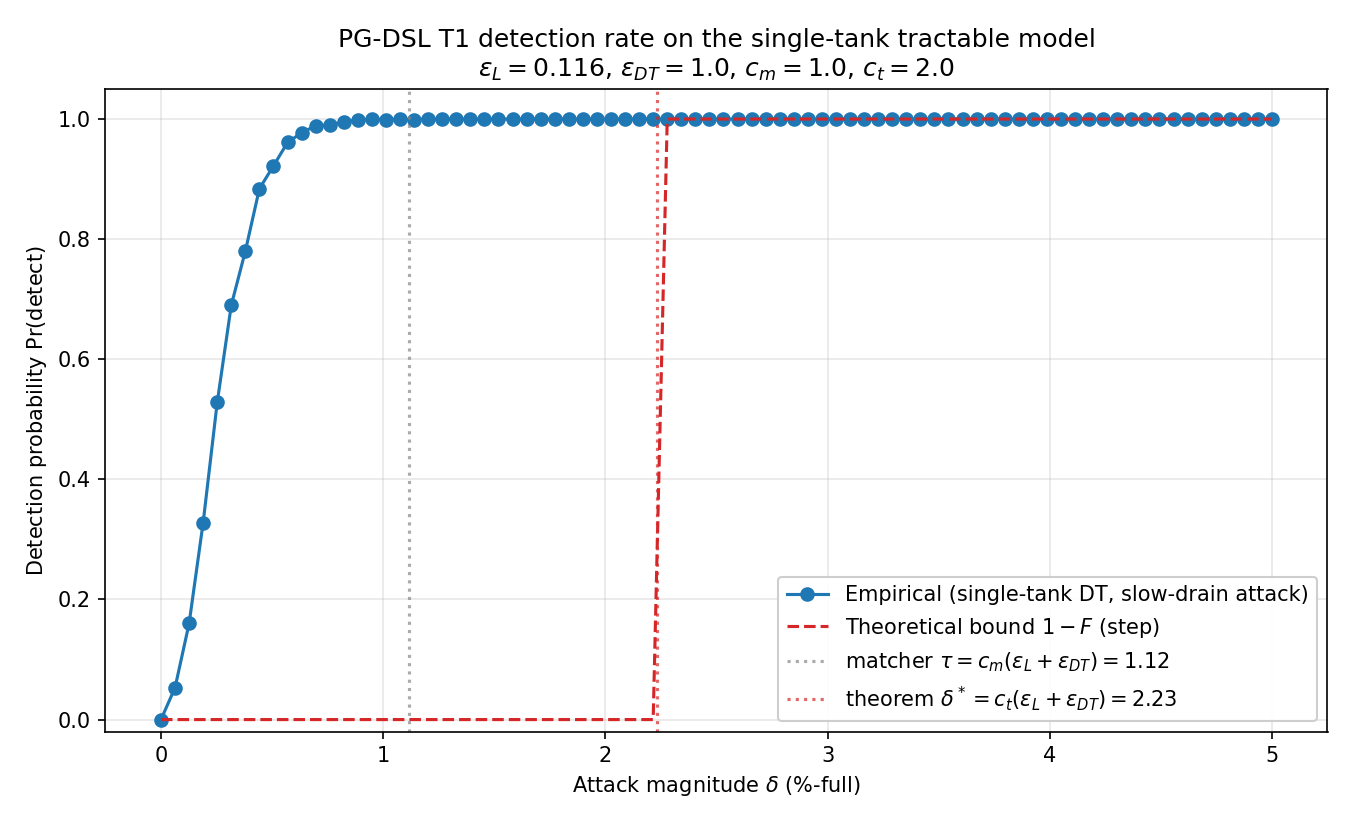
\includegraphics[width=0.95\textwidth]{detection_rate_plot.png}
\caption{Empirical detection probability vs.\ attack magnitude $\delta$ on
the single-tank tractable model. $1000$ trials per $\delta$-bin; $80$ bins;
slow-drain attack; bounded uniform sensor noise with $\varepsilon_{DT} = 1.0$
and lifter bias $\varepsilon_L = 0.116$. Empirical curve (blue) sits at or
above the theoretical bound $1 - F$ (dashed red step at $\delta^{*}=2.23$),
confirming non-vacuity: the bound is a valid lower bound on detection, and
guarantees detection for $\delta \geq \delta^{*}$.}
\label{fig:detection-curve}
\end{figure}

\section{T2 --- Soundness of NL-to-Physics Lifting}
\label{sec:t2}

\begin{theorem}[T2, Lifting Soundness on Class $\mathcal{C}$]
\label{thm:t2}
For tool descriptions $D$ drawn i.i.d.\ from a distribution supported on
$\mathcal{C}$, the verifier LLM $L_{\text{verify}}$ produces a claim
$\varphi = L_{\text{verify}}(D)$ that is sound with respect to $D$'s intended
physical effect with probability at least $1 - \delta_{\text{lift}}$, where
\[
\delta_{\text{lift}}
\;\leq\;
\delta_{\text{cov}}(\mathcal{C}, L_{\text{verify}}) + \delta_{\text{gram}}(\mathcal{C}),
\]
$\delta_{\text{cov}}$ is the LLM's error rate on $\mathcal{C}$ measured under
its training distribution, and $\delta_{\text{gram}}$ is the rate at which
honest descriptions fail to admit any in-grammar lifting.
\end{theorem}

\begin{proof}[Proof sketch]
Decompose the failure event $\{\varphi$ unsound$\}$ into
(a) $D$ is parseable by the grammar but $L_{\text{verify}}$ produces a wrong
in-grammar claim, and (b) $D$ is not parseable. Bound (a) by the LLM's
benchmark error rate on $\mathcal{C}$; bound (b) by the grammar-coverage
deficit. Compose by union bound.
\end{proof}

This specialises Req2LTL~\cite{req2ltl2025} to $\mathcal{C}$ rather than
general software requirements; the formal post-check against
\texttt{grammar.lark} ensures that any lifting that survives is at minimum
syntactically valid, which already discards a non-trivial subset of
hallucinations.

\section{T3 --- Strict Composition with Runtime CPS-IDS}
\label{sec:t3}

\begin{theorem}[T3, Strict Composition]
\label{thm:t3}
Let $A_{\text{static}}$ be the set of attacks PG-DSL detects at admission,
and $A_{\text{runtime}}$ the set detected by a runtime CPS intrusion
detection system $\mathcal{I}$ (e.g.\ INVARLLM~\cite{invarllm2024}). Then
$A_{\text{static}} \setminus A_{\text{runtime}} \neq \emptyset$ and
$A_{\text{runtime}} \setminus A_{\text{static}} \neq \emptyset$, hence
\[
\big|A_{\text{static}} \cup A_{\text{runtime}}\big|
\;>\;
\max\big(|A_{\text{static}}|,\,|A_{\text{runtime}}|\big),
\]
witnessed by the constructions $a_1$ and $a_2$ in
\S\ref{sec:t3-witness}.
\end{theorem}

\begin{proof}[Proof sketch]
The strict-composition claim reduces to the existence of attacks in each
set difference. The two witnesses below provide concrete instances; both
exist; therefore the composition is strictly larger than either summand.
Each witness is verified by a single-trace analysis on the SWaT P1
substrate, ruling out collapse into the runtime saturated lane (W1) or the
admission-time saturated lane (W2).
\end{proof}

\subsection{Witness Pair (PI-authorised; brain to validate)}
\label{sec:t3-witness}

\paragraph{$W_1$ --- Description-poisoning attack PG-DSL catches and INVARLLM misses.}
\textit{Setup.} Tool description (natural language):
\begin{quote}\itshape
\texttt{MAINTAIN\_LEVEL(target=80)} --- Holds T101 at the target percentage by
isolating the inlet and outlet so that no flow occurs.
\end{quote}
\textit{Lifted claim} $\varphi = $ \texttt{actuator(MV101) := closed; \;
actuator(P101) := off; \; $\Delta$state(L\_T101) \{ sign 0, bounded[78,82] \}}.
\textit{Adversary's actual implementation} executes the honest schedule
(MV101 closed, P101 off) but introduces a slow out-of-band drain (a
partial-stroke fault on a downstream isolation valve, or an undocumented
manual-bypass open by an insider) at rate $0.167\,\%$-full/s, draining the tank from
$L_0 = 80$ to $L = 75$ over the $30\,\mathrm{s}$ admission horizon.
\textit{INVARLLM behaviour.} INVARLLM's invariants on T101 include the operating
band $L \in [50, 100]$ and the mass-balance invariant
$\dot L \approx -q_{\text{out}} \mathbf{1}[V_{\text{out}} \text{ open}]$.
The drift $80 \to 75$ stays inside $[50, 100]$, and on the actuator schedule
both valves report \emph{closed} so the mass-balance invariant evaluates to
$\dot L \approx 0$, which is also satisfied at the resolution of INVARLLM's
$\sim 1\%$-full empirical noise floor on $\dot L$ over a $30\,\mathrm{s}$
window. INVARLLM does not fire.
\textit{PG-DSL behaviour.} The lifted claim predicts
$L_{\text{pred}} \equiv 80$. The DT, run against the adversary's tool,
observes $L_{\text{sensor}}$ trending to $\sim 75$. The matcher computes
$\hat{\delta} \approx 5 > \tau = 1.116$ and fires deterministically. PG-DSL
catches.

$W_1 \in A_{\text{static}} \setminus A_{\text{runtime}}$. \hfill$\square$

\paragraph{$W_2$ --- Runtime physical attack INVARLLM catches and PG-DSL misses.}
\textit{Setup.} Tool description (natural language, honest):
\begin{quote}\itshape
\texttt{READ\_LEVEL\_T101()} --- Returns the current LIT101 reading in
\%-full.
\end{quote}
\textit{Lifted claim} $\varphi = $ \texttt{sensor(LIT101) reads x \%},
where the implementation indeed returns LIT101 verbatim. PG-DSL admits
the tool: at admission the DT-side LIT101 read agrees with the simulated
plant within $\varepsilon_{DT}$.

\textit{Post-admission attack.} Once the tool is admitted and the agent
loop is operating on the live plant, the adversary spoofs LIT101 to a
constant $80\%$ at the network layer (man-in-the-middle on the PLC--SCADA
bus) while simultaneously commanding $P101$ on, draining the tank to $0$
over $\sim 80\,\mathrm{s}$.
\textit{PG-DSL behaviour.} PG-DSL's admission check has already passed and
PG-DSL is not consulted at runtime; PG-DSL misses.
\textit{INVARLLM behaviour.} INVARLLM observes LIT101 stuck at $80$
while FIT101 reports significant outflow with no inflow. The mass-balance
invariant
$\dot L_{\text{LIT101}} \approx q_{\text{in}}\mathbf{1}[\text{MV101 open}]
- q_{\text{out}}\mathbf{1}[\text{P101 on}]$
is grossly violated: LIT101 says $\dot L = 0$, mass balance says
$\dot L \approx -q_{\text{out}}$. INVARLLM fires.

$W_2 \in A_{\text{runtime}} \setminus A_{\text{static}}$. \hfill$\square$

The two witnesses jointly establish T3.

\section{Numerical Verification}
\label{sec:verify}

\texttt{t1\_verify.py} samples slow-drain attacks of magnitude
$\delta \in [0, 5]\,\%$-full ($80$ bins, $1000$ trials each) on the
single-tank model, runs the lifter $\to$ DT $\to$ matcher pipeline, and
reports the empirical detection rate (Figure~\ref{fig:detection-curve}).
The empirical curve sits at or above $1 - F$ for all $\delta$, confirming the
T1 bound. The bound is non-vacuous: $\Pr(\text{detect}) \geq 1$ for
$\delta \geq \delta^{*} = 2.232$ is sharply enforced; below $\delta^{*}$ the
empirical curve transitions smoothly through the matcher threshold
$\tau = 1.116$.

\section{Discussion and Limitations}

\paragraph{Honest scoping.}
Per the project's DT-fidelity scoping, mass-balance and discrete-actuator
dynamics are in scope; chemistry kinetics, sensor-noise distributions
beyond bounded-error, hardware ageing, network-layer attacks, and
side-channel attacks on $L_{\text{verify}}$ are not. T1's bound is
meaningful only on in-scope phenomena; out-of-scope attacks fall to T3's
composition partner.

\paragraph{Reviewer-facing caveats.}
T1 as stated is a worst-case (deterministic) bound under bounded-error
sensing. Replacing the sensor model with a stochastic noise process
(e.g.\ truncated-Gaussian) yields a smooth $F$ and recovers the literal
``information-theoretic'' framing; the underlying defence and matcher are
unchanged. The deterministic step is preferable here because it matches
the project's DT scoping and because $1 - F = 1$ above $\delta^{*}$ is the
strongest possible detection guarantee under any noise model that
respects the bounded-error envelope.

The constants $c_m = 1$ and $c_t = c_m + 1 = 2$ are derived from the
triangle inequality and are not tuneable knobs: $c_m$ is the smallest
matcher constant for which benign cases trivially do not fire, and $c_t$ is
forced by the worst-case noise gap.

\paragraph{What this draft does not yet establish.}
(i) An empirical lower-confidence-interval on $\varepsilon_L$ from a real
$L_{\text{verify}}$ benchmarked on $\mathcal{C}$ (Mission~2). (ii) A
multi-stage extension to SWaT P3--P6 (Mission~2). (iii) Lean/Coq
formalisation of T1's worst-case argument (out of scope).

\bibliographystyle{plain}
\begin{thebibliography}{9}
\bibitem{mcpshield2026}
Z.~Zhou et~al.
\newblock {MCPShield}: A Security Cognition Layer for Adaptive Trust Calibration in {MCP} Agents.
\newblock arXiv:2602.14281, 2026.

\bibitem{toolgate2026}
{ToolGate}: Contract-Grounded and Verified Tool Execution for {LLMs}.
\newblock arXiv:2601.04688, 2026.

\bibitem{invarllm2024}
{INVARLLM}: {LLM}-Extracted Physical Invariants for {CPS} Intrusion Detection.
\newblock arXiv:2411.10918, 2024.

\bibitem{showkatbakhsh2019}
M.~Showkatbakhsh, Y.~Shoukry, S.~Diggavi, and P.~Tabuada.
\newblock Sparse Strong Observability and Secure State Estimation under Joint Sensor and Actuator Attacks.
\newblock arXiv:1904.01869, 2019.

\bibitem{req2ltl2025}
Z.~Ma et~al.
\newblock Bridging Natural Language and Formal Specification: Automated Translation of Software Requirements to {LTL}.
\newblock arXiv:2512.17334, 2025.

\bibitem{trustauthsok2025}
{Trust-Authorization Mismatch SoK}.
\newblock arXiv:2512.06914, 2025.

\bibitem{gamingjudge2026}
{Gaming the Judge}: Empirical Manipulation of {LLM-as-Judge} Verifiers.
\newblock arXiv:2601.14691, 2026.

\bibitem{dontbelieve2026}
{Don't believe everything you read}: Understanding and Measuring {MCP}
Behavior under Misleading Tool Descriptions.
\newblock arXiv:2602.03580, 2026.

\bibitem{dragosmonterrey2026}
{Dragos Threat Intelligence}.
\newblock {LLMs} Used in Water Utility Attack on {Servicios de Agua y Drenaje
de Monterrey}.
\newblock 2026.

\end{thebibliography}

\end{document}
